\section{Practical exercice: Polynomial evaluation}

Polynomial evaluation is a common source of computational error. Polynomials are frequently used for function interpolation in libraries or user codes. As we will see, different evaluations of the same polynomial do not have the same behavior in terms of performance or numerical accuracy.

This tutorial uses the Tchebychev polynomial from ~\cite[pp.52-54]{parker1997monte}:

$$T(x)=\sum_{i=0}^{10}{a_i \times x^{2i}}$$
With:
$a_i \in [
  1,
  \matminus 200,
  6600,
  \matminus 84480,
  549120,
  \matminus 2050048,
  4659200,
  \matminus 6553600,
  5570560,
  \matminus 2621440,
  524288
]$

We are interested in evaluating  $T$ near $1$ as discussed in~\cite[pp.52-54]{parker1997monte}.

\subsection{Evaluation of the naive form}

\subsubsection{First steps with Verificarlo}

In this first approach, we will evaluate the polynomial in its naive form and in single precision. This part of the tutorial is located in the \texttt{tchebychev/} folder.

\begin{question}
  \begin{enumerate}[(a)]
  \item Open the {\tt tchebychev.c} file and observe the function {\tt REAL expanded(REAL x)}.

  \item Compile {\tt tchebychev.c} with {\tt verificarlo} using the following command:
\begin{verbatim}
verificarlo -D FLOAT tchebychev.c -o tchebychev
\end{verbatim}
  \item Run the program.
  \end{enumerate}
\end{question}

You should get an error as the \texttt{VFC\_BACKENDS} environment variable is empty.
The simplest backend is the one emulating IEEE-754 arithmetic(\texttt{libinterflop\_ieee.so}). 
It has a \texttt{-{}-debug} option that trace each instrumented floating-point operations.

\begin{question}
Run the program using the IEEE backend,
\begin{verbatim}
VFC_BACKENDS="libinterflop_ieee.so --debug" ./tchebychev 0.99 EXPANDED
\end{verbatim}
\end{question}

To estimate the numerical error, we will now use the Monte Carlo Arithmetic backend
(\texttt{libinterflop\_mca.so}) in single precision by simulating round-off errors that could occurs at 24 bits of precision.

\begin{question}
  \begin{enumerate}[(a)]
  \item Run the program using the Monte Carlo Arithmetic backend with 24 bits precision,
\begin{verbatim}
VFC_BACKENDS="libinterflop_mca.so --precision=24" ./tchebychev 0.99 EXPANDED
\end{verbatim}
  \item Execute the program multiple times. What can you observe?
  \end{enumerate}
\end{question}

Monte Carlo arithmetic backend supports different modes,
\begin{itemize}

  \item \texttt{-{}-mode=rr} is the \emph{random round} mode that adds noise on the
    result of an operation only when the operation is not exactly representable
    at the chosen precision. This mode is useful to simulate the effect of
    round-off errors.

  \item \texttt{-{}-mode=pb} is the \emph{precision bound} mode that adds noise on
  the operands before performing the operation. It is useful to simulate the
    effect of cancellations errors.

  \item \texttt{-{}-mode=mca} is the default mode that combines \texttt{rr} and
  \texttt{pb} modes.

\end{itemize}

\begin{question}
  \begin{enumerate}[(a)]
  \item Now recompile with verificarlo the program in double precision using the command:\newline
    {\tt verificarlo -D DOUBLE tchebychev.c -o tchebychev} \\
  \item Execute the program with arguments \texttt{0.99 EXPANDED} with the Monte Carlo arithmetic backend. Try different precisions such as 53, 24, 10. Try also to use different modes (rr, pb, mca). What do you observe?
  \end{enumerate}
\end{question}

\subsubsection{Numerical quality analysis}

In this section, we analyze the numerical quality of the computed results based on the naive version of the given polynomial. 
You can rely on the \texttt{run.sh} script available in the exercice directory which automates the required verificarlo runs. 
Visualization is done using the \texttt{plot.py} script.

Since we are working with a headless docker image, the \texttt{plot.py} output
will be a \texttt{.pdf} file that you can open in the host machine.


\begin{question}
  \begin{enumerate}[(a)]
 \item Open {\tt run.sh} and understand how it works.
  \item Modify {\tt run.sh} to evaluate the polynomial in the interval $[0.5,1]$ by $0.001$ step (you can leave the number of execution unchanged).
  \item Open {\tt plot.py} and understand how it works, and what are the plotted data.
  \end{enumerate}
\end{question}

Figure~\ref{fig:exp_hor_24_53} is generated with the \texttt{plot.py} script.

The lowest part of each plot shows the $T(x)$ samples and their average in dotted line. The 20 Monte Carlo samples $T(x)$ are plotted for each $x$ value (sometime overlapping on the graphic).
The central part is the empirical standard deviation $\hat\sigma$ for each value of $x$.
The upper part of the figure represents the number $s$ of significant digits of each output: $s=-\log_{10}\left|\dfrac{\hat\sigma}{\hat\mu}\right|$ with $\hat\sigma$ the sample empirical standard deviation and $\hat\mu$ their average.

\begin{question}
\begin{enumerate}[(a)]
\item To execute the {\tt EXPANDED} version with {\tt DOUBLE} and a virtual precision of 24 bits, execute the command: {\tt ./run.sh EXPANDED
      DOUBLE 24 mca} \newline This command's output is given in figure~\ref{fig:exp_hor_24_53} (Top Left).
  \item With a virtual precision of 53, execute the command: {\tt ./run.sh EXPANDED DOUBLE 53 mca} \newline
  This command's output is given in figure~\ref{fig:exp_hor_24_53} (Top Right).
  \item Compare the number $s$ of significant digits in both case. What is the problem and is double precision a solution?
  \end{enumerate}
\end{question}

\begin{table}
\begin{tabular}{cc}
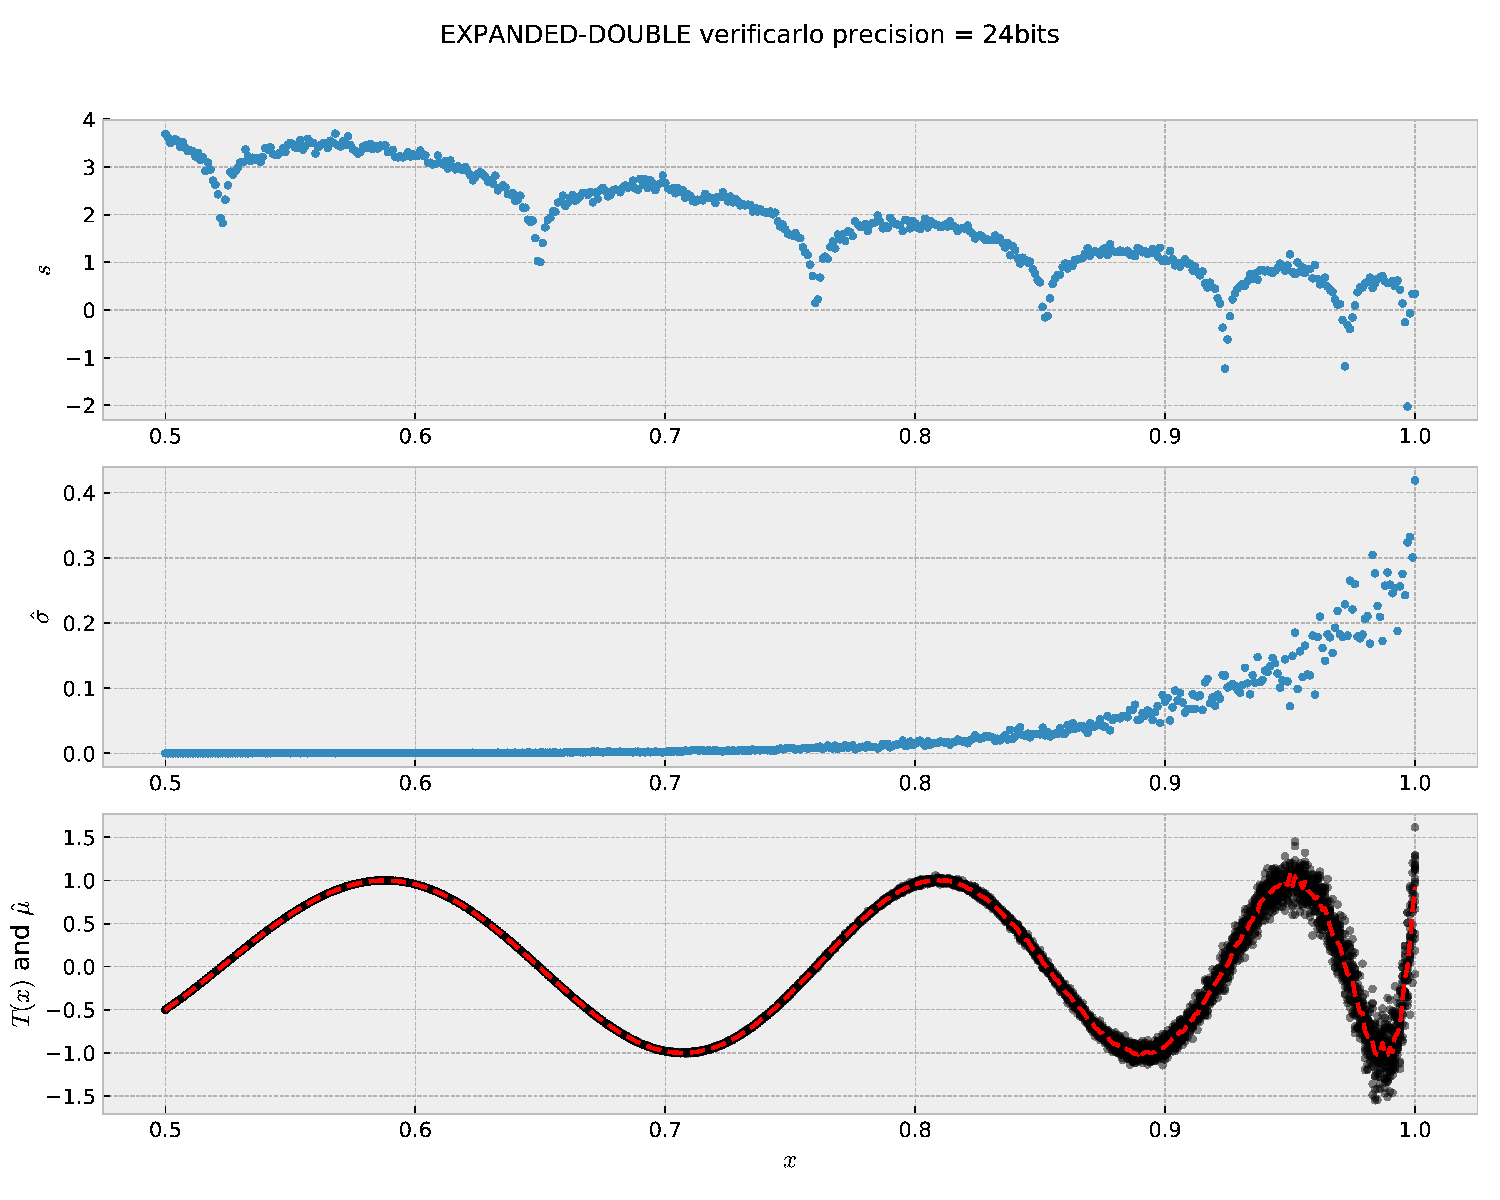
\includegraphics[width=.47\textwidth]{EXPANDED-DOUBLE-24.pdf} &
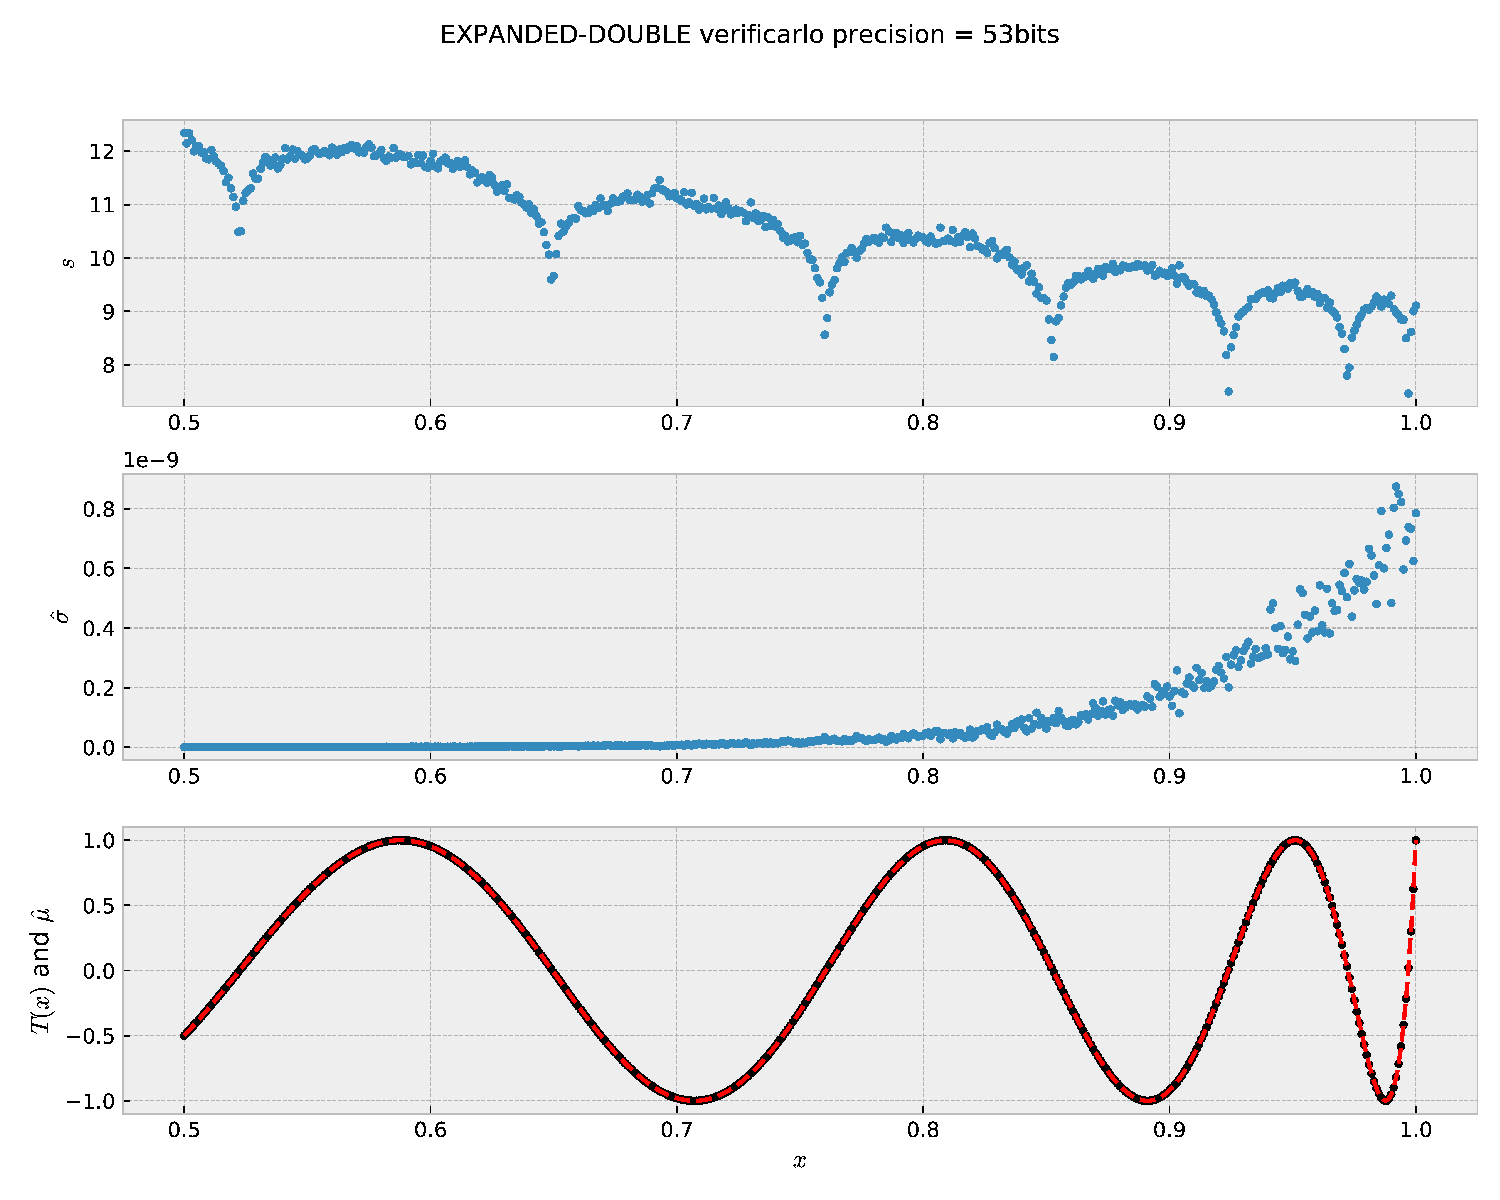
\includegraphics[width=.47\textwidth]{EXPANDED-DOUBLE-53.pdf} \\
%Expanded form, 24 bits & Expanded form, 53 bits \\
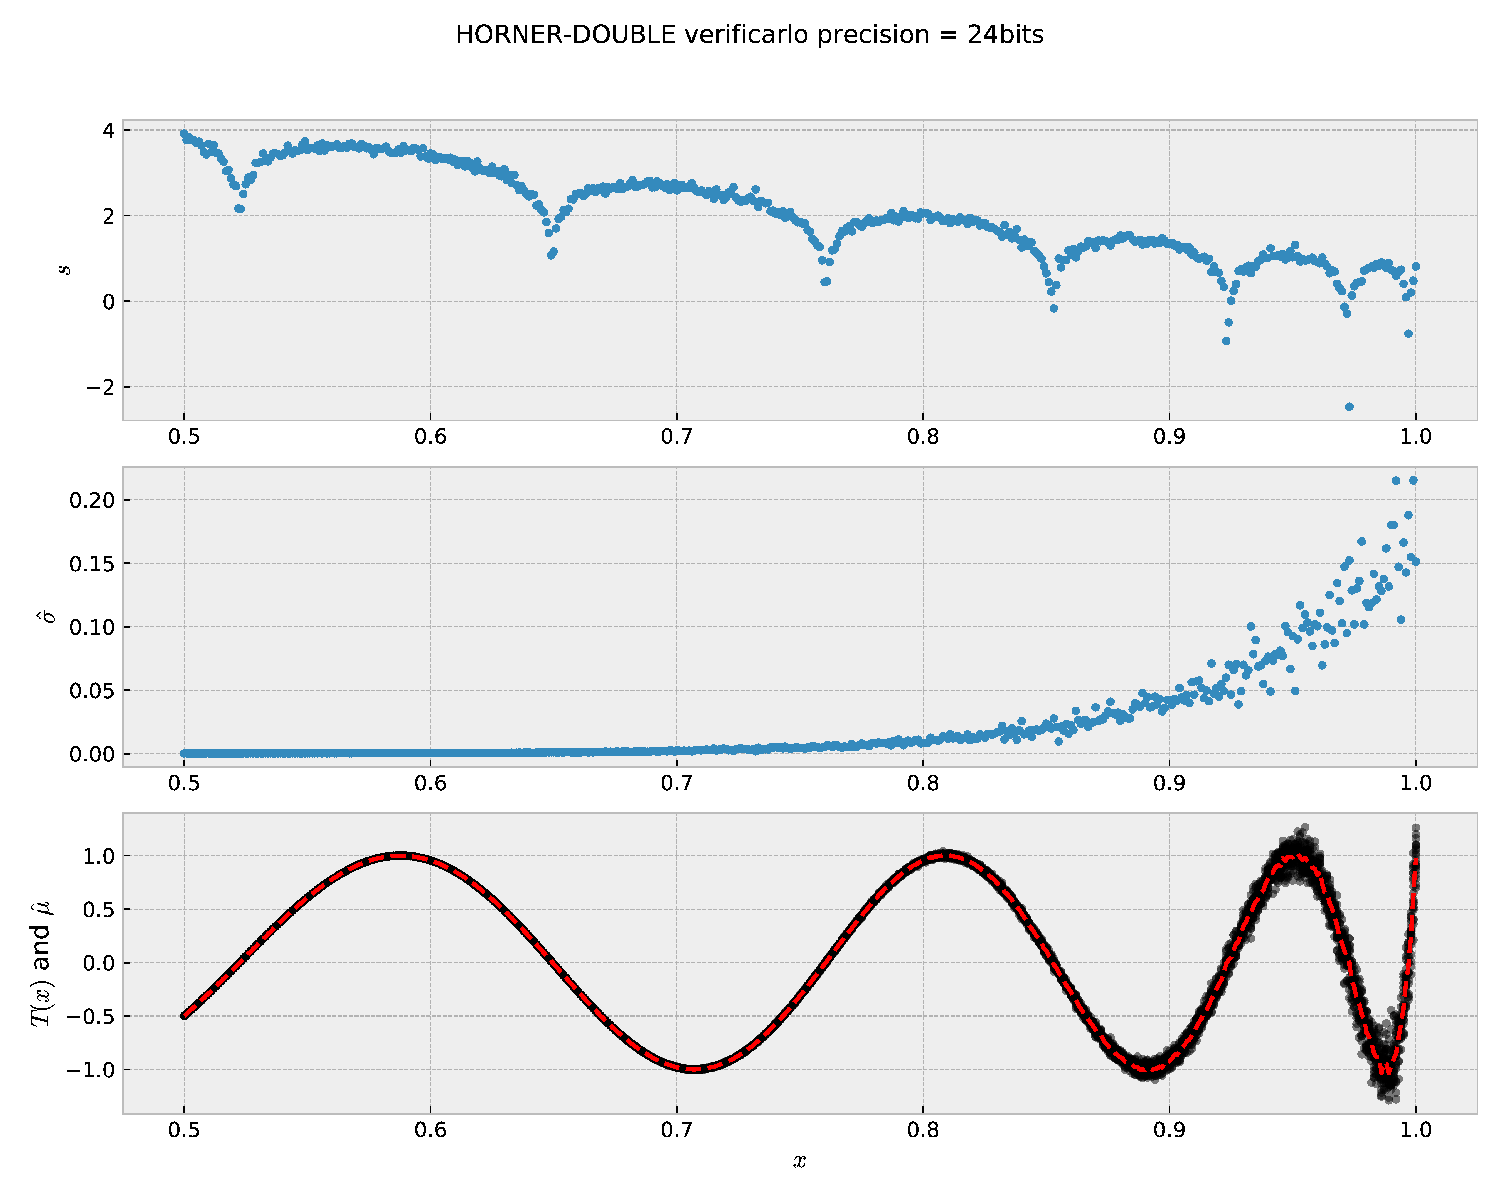
\includegraphics[width=.47\textwidth]{HORNER-DOUBLE-24.pdf} &
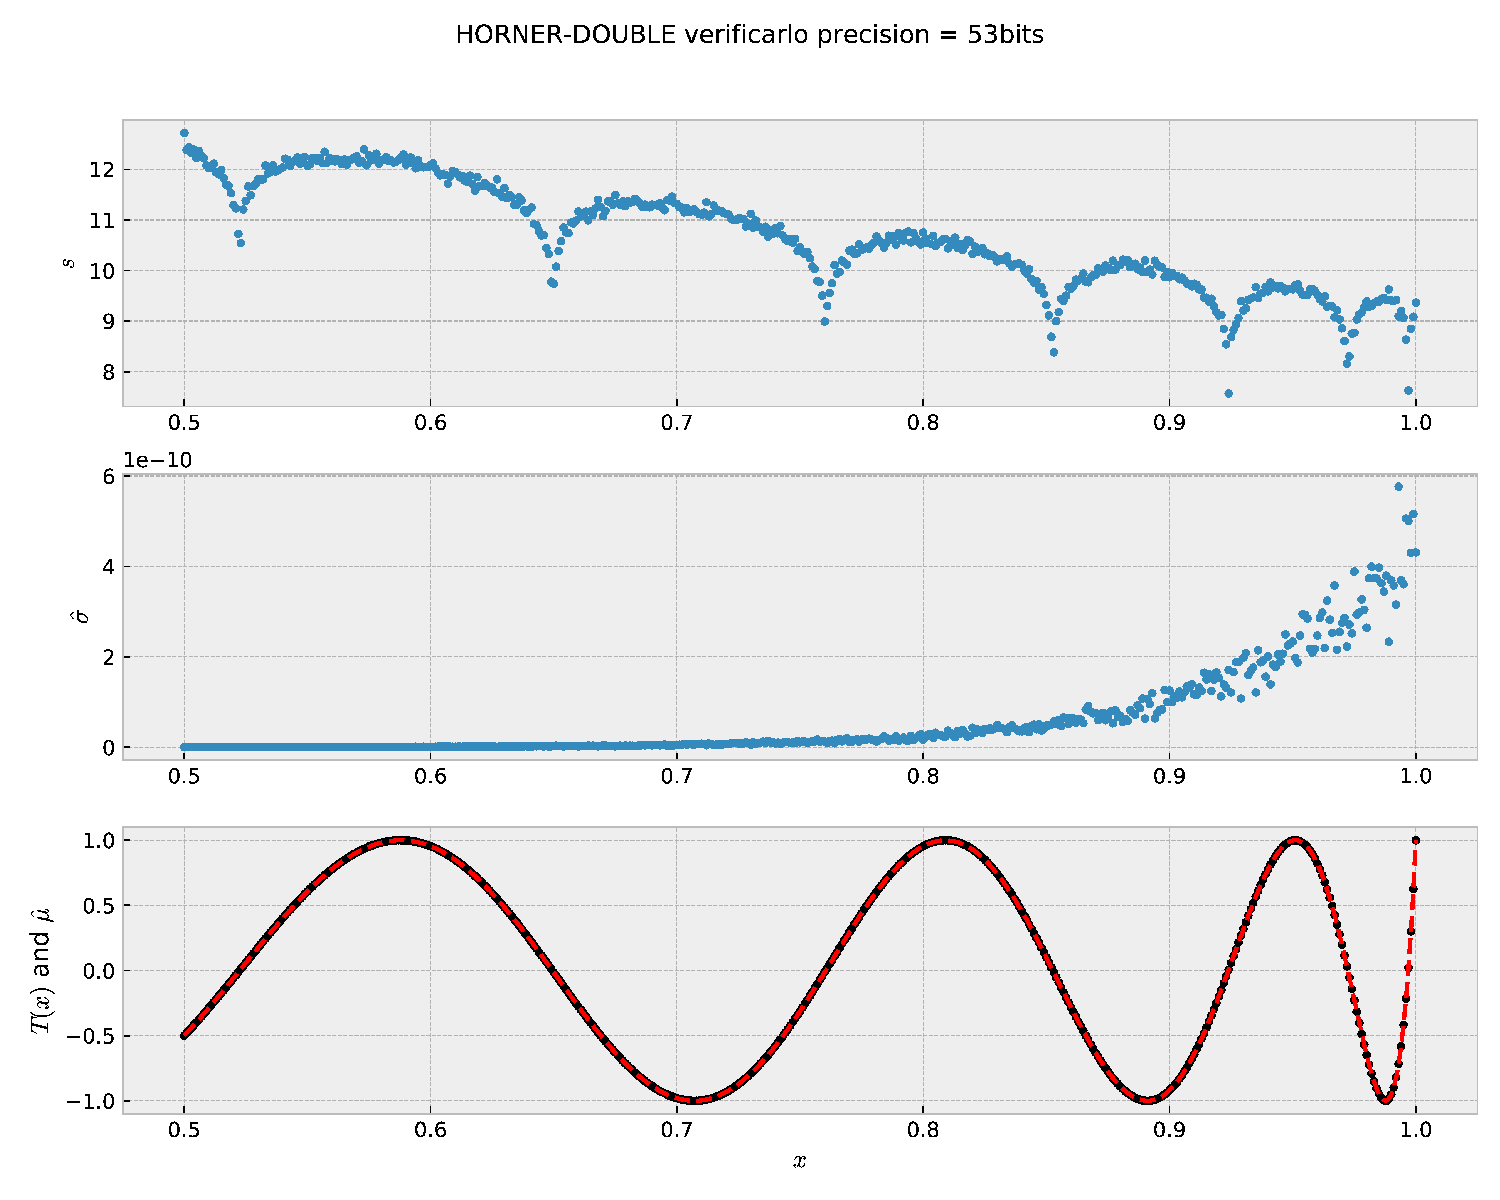
\includegraphics[width=.47\textwidth]{HORNER-DOUBLE-53.pdf} \\
%Horner form, 24 bits & Horner form, 53 bits \\
\end{tabular}
  \caption{Evaluation of T(x) in its \{Expanded/Horner\} form, compiled in double precision, with a virtual precision of \{24/53\} bits}
  \label{fig:exp_hor_24_53}
\end{table}


One can notice that the polynomial evaluation done with 24 bits is subject to severe {\it cancellations} when the input value is close to $1$.
This drasticaly reduces the accuracy of the result.
Using evaluation in double precision on the contrary seems satisfactory...
But this solution forces the developer to use a larger and more expensive data type and it does not solve the problem, it only delays it.

\FloatBarrier

\subsection{Evaluation using Horner's method}
There exists multiple ways to evaluate polynomials, using associativity, commutativity and factorization.
Each evaluation scheme has its own impact on precision and performance.
One of them has already been the subject of many studies: the Horner's method which for the considered polynomial take the following form:

\[
	T(x) = (\dots((a_n\times x^2 + a_{n-1})\times x^2 + a_{n-2})\dots) \times x^2
    + a_0
\]

$$T(x) = (((((((((524288*x^2-2621440)*x^2+5570560)*x^2-6553600)*$$
$$x^2+4659200)*x^2-2050048)*x^2+549120)*x^2-84480)*$$
$$x^2+6600)*x^2-200)*x^2+1$$

\begin{question}
  \begin{enumerate}[(a)]
  \item Open the file {\tt tchebychev.c} and have a look to the function {\tt REAL horner(REAL x)}
\item While keeping previous execution parameters, execute the command {\tt ./run.sh HORNER DOUBLE 53 mca}  \newline The output of this command is given in figure~\ref{fig:exp_hor_24_53} (Bottom Left).
  \end{enumerate}
\end{question}

\begin{question}
\item Execute the command {\tt ./run.sh HORNER DOUBLE 24 mca}  \newline
The output of this command is given in figure~\ref{fig:exp_hor_24_53} (Bottom Right).
What do you observe?
\end{question}

As shown in this experiment, the improvment brought by the Horner scheme is not significant ($\simeq$ 1 additional significant bit in the result). 
 However, it minimizes the
number of operations and allows to use the FMA ({\it Fused Multiply Add}). For
a polynomial of degree $n$, it produces $n-1$ FMA. Moreover, when doing
multiple independent evaluations it can be vectorized.

